\documentclass[UTF8, letter]{article}

\usepackage[margin=1in]{geometry}
\usepackage{graphicx}
\usepackage{lipsum}
\usepackage[framemethod=tikz]{mdframed}
\usepackage{minted}
\usepackage{setspace}
\usepackage{xcolor}
\usepackage{subcaption}
\usemintedstyle{xcode}

\definecolor{codebg}{RGB}{192,199,209}
\definecolor{outputbg}{RGB}{243,244,248}

\mdfdefinestyle{codeframe}{
	backgroundcolor=codebg,
	linewidth=0,
	skipbelow=-10
}

\mdfdefinestyle{outputframe}{
	backgroundcolor=outputbg,
	linewidth=0,
	skipbelow=-10
}
\newmdenv[style=codeframe,%
	settings={\singlespacing}]{codeblock}
	
\newmdenv[style=outputframe,%
	settings={\singlespacing}]{outputblock}

\title{Programming Assignment 3 \\
\large INFO-5502 (Section 002): \\
Analytic Tools, Techniques and Methods }
\author{Ramandeep Harjai}


\begin{document}
\maketitle

\doublespacing
\setlength{\parskip}{\baselineskip}
\setlength{\parindent}{4em}

\begin{flushleft}
\noindent
Import required Python packages.
\end{flushleft}

\begin{codeblock}
\begin{minted}{python}
import matplotlib.pyplot as plt
import matplotlib.patches as pth
from random import seed
from random import random
from random import uniform
from random import randint
import math
import numpy as np
\end{minted}
\end{codeblock}


\begin{flushleft} \noindent
Function: \texttt{randomCoordinate()} generates a pair of random coordinates (x, y) between a set of two given coordinates: x\textsubscript{1}, y\textsubscript{1}, and x\textsubscript{2}, y\textsubscript{2}.
\linebreak
\textbf{Arguments}: (1) \texttt{xLowLimit}: x coordinate for lower bound, (2) \texttt{xHighLimit}: x coordinate for higher bound, (3) \texttt{yLowLimit}: y coordinate for higher bound, (4) \texttt{yHighLimit}: y coordinate for higher bound. 
\linebreak
\textbf{Returns}: random x, y coordinate
\end{flushleft}

\begin{codeblock}
\begin{minted}{python}
def randomCoordinate(xLowLimit:int, xHighLimit:int, 
                     yLowLimit:int, yHighLimit:int)->(int, int):
  ''' Generates a random floating-point coordinate 
      between two sets of coordinates provided. 
      Returns:
        - (x,y): Random Coordinate'''
  return((uniform(xLowLimit, xHighLimit),
          uniform(yLowLimit, yHighLimit)))
\end{minted}
\end{codeblock}

\pagebreak

\begin{flushleft} 
\noindent
Function: \texttt{pointInCircle()} validates if a given point exists within a given circle.
\linebreak
\textbf{Arguments}: (1) \texttt{xPoint}: x coordinate of the point to be tested, (2) \texttt{yPoint}: y coordinate of the point to be tested, (3) \texttt{xCircle}: x coordinate for the center of the circle, (4) \texttt{yCircle}: y coordinate for the center of the circle, (5) \texttt{rCircle}: radius for the circle.
\linebreak
\textbf{Returns}: \texttt{True}: if the given point exists within the given circle. \texttt{False}: if the given point exists within the given circle. 
\end{flushleft}

\begin{codeblock}
\begin{minted}{python}
def pointInCircle(xPoint:int, yPoint:int, 
                  xCircle:int, yCircle:int, rCircle:int)->bool:
  ''' Test if a given point (x,y coordinate) lies within a 
      Circle of given center point, and radius.
      Returns: 
        - True: if point lies within the circle
        - False: if point lies outside the circle '''                  
  d = math.sqrt(pow((xPoint-xCircle),2) + pow((yPoint-yCircle),2))
  if d <= rCircle:
    return True
  else:
    return False
\end{minted}
\end{codeblock}

\begin{flushleft} 
\noindent
\texttt{Main program}: runs Monte Carlo simulation for 15 different number of iterations (1 | 10 | 50 | 100 | 250 | 500 | 1,000 | 2,500 | 5,000 |  10,000 | 20,000 | 40,000 | 80,000 | 100,000 | 200,000). For each iteration, the program (1) generates corresponding number of random x,y coordiantes, (2) determines whether the point belongs within the circle or square, (3) plots the coordinates as a point on a chart, and (4) calculates the value of pi.
\end{flushleft}

\begin{codeblock}
\begin{minted}{python}
# graph coordinates & settings
originX:int = 1
originY:int = 1
radius:int = 6
pointSize = 0.5
sqColor = '#1192e8'
crColor = '#fa4d56'

# number of iterations for Monte Carlo simulation
iterations=[1, 10, 50, 100, 250, 500, 1000, 2500, 5000, 
            10000, 20000, 40000, 80000, 100000, 200000]

# list to store computed pi-values
pi_results = []

# draw graph
plotCols:int = 3
plotRows:int = int(len(iterations)/plotCols)
figure, ax = plt.subplots(plotRows, plotCols, constrained_layout=True)
figure.set_dpi(150)
rowCounter = 0
colCounter = 0
for iteration in iterations:
  print('Running simulation with {} iterations...'.format(iteration))
  # draw square
  square = pth.Rectangle((originX,originY),
                        radius*2, radius*2,
                        linewidth=1, 
                        edgecolor=sqColor,
                        fill=False)
  # draw circle
  circle = pth.Circle((originX+radius,originY+radius),
                      radius, edgecolor=crColor, 
                      linewidth=1, fill=False) 
  
  ax[rowCounter, colCounter].add_patch(square)
  ax[rowCounter, colCounter].add_patch(circle)


  # compute & draw random points for Monte Carlo simulation
  nInnerPoints = 0
  piValue = 0
  for _ in range(iteration):
    xCord, yCord = randomCoordinate(originX,(radius*2)+1,originY,(radius*2)+1)
    if pointInCircle(xCord, yCord, originX+radius, originY+radius, radius):
      ax[rowCounter, colCounter].scatter(xCord,yCord,s=pointSize,c=crColor)
      nInnerPoints += 1
    else:
      ax[rowCounter, colCounter].scatter(xCord,yCord,s=pointSize,c=sqColor) 

  # compute pi-value and store in results
  piValue = 4 * (nInnerPoints/iteration)
  pi_results.append((iteration, piValue))

  # draw sub-plot for the current iteration
  ax[rowCounter, colCounter].set_title('n={}\npi={}'.format(iteration, 
                                                            piValue), 
                                       fontsize= 8)
  ax[rowCounter, colCounter].set_xticks([])
  ax[rowCounter, colCounter].set_yticks([]) 
  ax[rowCounter, colCounter].relim()
  ax[rowCounter, colCounter].autoscale_view()      

  # manage sub-plot position in the grid
  colCounter += 1
  if (colCounter % plotCols == 0):
    colCounter = 0
    rowCounter += 1

plt.show()
\end{minted}
\end{codeblock}

\begin{flushleft} \noindent
\texttt{Output}: for Monte Carlo simulation for 15 different iterations.
\end{flushleft}

\begin{outputblock}
\begin{minted}{python}
Running simulation with 1 iterations...
Running simulation with 10 iterations...
Running simulation with 50 iterations...
Running simulation with 100 iterations...
Running simulation with 250 iterations...
Running simulation with 500 iterations...
Running simulation with 1000 iterations...
Running simulation with 2500 iterations...
Running simulation with 5000 iterations...
Running simulation with 10000 iterations...
Running simulation with 20000 iterations...
Running simulation with 40000 iterations...
Running simulation with 80000 iterations...
Running simulation with 100000 iterations...
Running simulation with 200000 iterations...
\end{minted}
\end{outputblock}

\centering
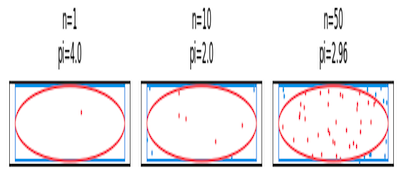
\includegraphics[width=\textwidth]{output-1-1.png}
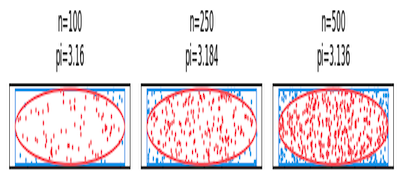
\includegraphics[width=\textwidth]{output-1-2.png}

\includegraphics[width=\textwidth]{output-1-3.png}
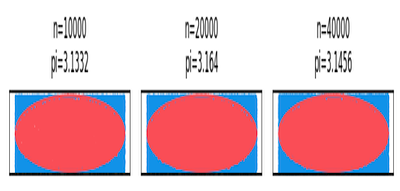
\includegraphics[width=\textwidth]{output-1-4.png}
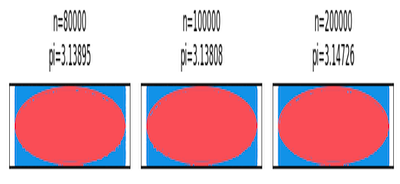
\includegraphics[width=\textwidth]{output-1-5.png}

\begin{flushleft} \noindent
The code snippet below outputs the 15 different pi-values computed using 15 different iterations of Monte Carlo simulation.
\end{flushleft}

\begin{codeblock}
\begin{minted}{python}
print("pi-values computed using Monte Carlo simulation: ")
for pi in pi_results:
  print(pi[1])
\end{minted}
\end{codeblock}

\begin{outputblock}
\begin{minted}{python}
pi-values computed using Monte Carlo simulation:
4.0
2.0
2.96
3.16
3.184
3.136
3.144
3.0752
3.1304
3.1332
3.164
3.1456
3.13895
3.13808
3.14726
\end{minted}
\end{outputblock}

\pagebreak
\begin{flushleft} \noindent
The code snippet below generates a line chart for 15 different pi-values computed using 15 different iterations of Monte Carlo simulation.
\end{flushleft}

\begin{codeblock}
\begin{minted}{python}
figure, ax = plt.subplots(constrained_layout=True)
figure.set_dpi(150)
ax.plot(*zip(*pi_results), lw=1, c='black', alpha=0.6, 
		label='Monte Carlo Simulation')
ax.set_title('Value of π (pi) using Monte Carlo simulation'
		.format(iteration, piValue), fontsize= 12)
ax.set_xlabel('Iterations')
ax.set_ylabel('Value of π (pi)')
plt.plot([-10000, 210000], [3.14159, 3.14159], 'r:', lw=1, 
			label='π = 3.14159')

plt.ylim([2.0, 4.2])
plt.legend()
plt.show()		
\end{minted}
\end{codeblock}

\begin{center}
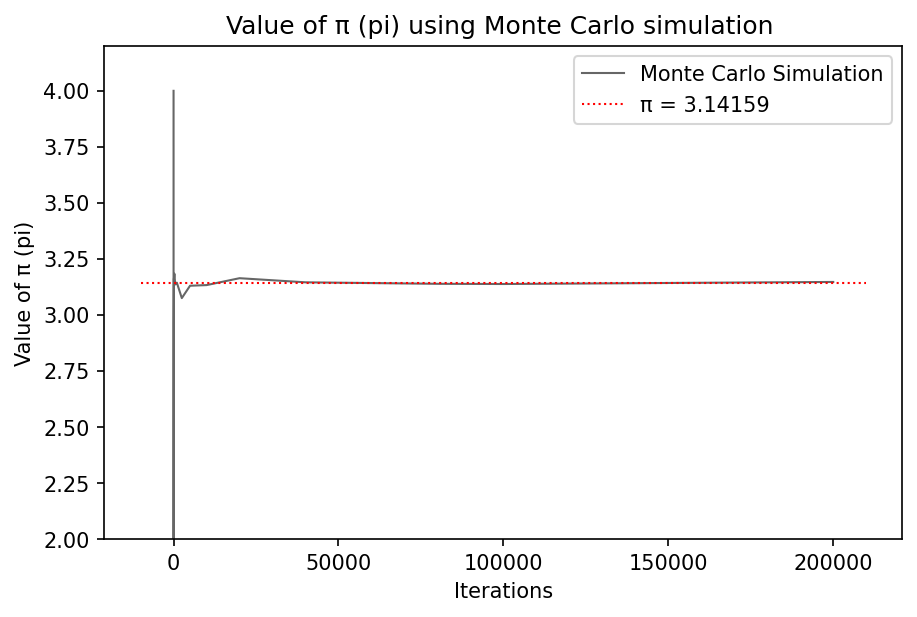
\includegraphics[width=\textwidth]{output-2.png}
\linebreak
\linebreak	
***** \textit{end of document} *****
\end{center}

\end{document}
